% --------------------------------------------------------------------

\section{Introduction}

Communicating with each other using technologies, such as Bluetooth, is becoming ever more popular in the field. Both old and new emerging technologies enable us to create new ways of establishing communication between total strangers with similar interests. This thesis describes how these technologies can be used to create social interaction between strangers and therefore increase their well-being of people and their performance during sports.

Familiar strangers is a concept first introduced by the psychologist Stanley Milgram in 1972 in his essay \citep{milgram1992}. We often come across to the same strangers while doing sports, but do not interact with them. These people, that you have met frequently but never interacted with, are called familiar strangers. \citep{familiarStranger}. Familiar strangers as a concept isn't limited to sports, but targeting the research to people who have similar interests (sports) by definition makes monitoring of their behavior simpler. While social networking between strangers has been research before, this concept of social interaction between familiar strangers in sports, is new in the field.

Methods used in this paper to research this problems are:
\begin{itemize}
\item  Literature review.
\item Conducting interviews.
\item Creating a prototype application for research data.
\end{itemize}

This paper presents a prototype Android application that will log the times strangers passing by you. When you come across to a strangers enough times, the application will suggest communication with the stranger. With the prototype, you can view where and how many times you have encountered that person and what are they interested in. Interesting questions related to this prototype application are, whether users are willing to establish communication based on similar interest and similar real-life habits (sports routes and times) and also how much information users are willing to share to total strangers. Data gathered form this prototype application can later be used to verify assumptions about the users behavior and to learn new information. The prototype application takes privacy seriously and is quite conservative about sharing information. The level of privacy can later then be modified based on feedback from the users.

The application uses Bluetooth beacons to identify the strangers and log the encounters to a web server. This enables the users to interact with the strangers also outside the sports activity itself. They don't have to approach the strangers while doing sports but they can later on interact with people they have met along the way and find similar interests with. 

The interviews were composed from open-ended questions where the goal was more to find new information rather than just to validate previous assumptions. The interviews were extensive and performed only for a handful of possible end users of the application. No survey's were conducted for this thesis.

\section{Related work}

This section presents related works from multiple perspectives: the social interaction perspective, the perspective of doing sports, social sports and also about related technology used in the thesis. The design and implementation of the prototype application relies on results from this section.

\subsection{Social interaction}

Getting to know strangers and finding people to do sports with can be a daunting task especially for people who have just moved to a new city or a country. It is important to make finding strangers as easy as possible with the use of modern technology without compromising the privacy of the users.

\cite{socialAdHoc} studied ad hoc social networking with a social networking system called TWIN. In a survey conducted after the study, the method for approaching unfamiliar persons was one of the highest rated features of the system. \cite{mobileMatchmaking} conducted a survey where 90\% of the participants stated that they would use regularly a service which would help introduce nearby strangers to each other. Serendipity, the application created for their research, is a mobile match-making system which alerts users when someone with similar interests comes into proximity. The reactions to the system have been overwhelmingly positive. These results imply that systems which allow people to interact with familiar strangers are in fact desired by users. The users were also less worried about their privacy than perhaps was anticipated by the researchers. No major problems were found in being able to interact with strangers in the research.

\subsection{Sports}

Meeting strangers is only one part of the assumed benefits of the prototype application. One of the goals for the application is to encourage people to exercise more. \citep{foundations} present how participating in sports improves us in various physical and social ways.

Research done by \citep{joggingTheDistance} also suggests that doing sports with another person on a similar level of fitness can create and enhance social relationships between them. Therefore, finding a partner to do sports with benefits people and might result in better performance and motivation to do sports.

One of the problems in creating the application is to figure out that how frequently people doing sports actually meet familiar strangers. Setting the level of passing by's before allowing users to communicate with each other affects the whole user experience of the prototype application. One problem is also that do, for example joggers use the same route always or do they change it often. Changing the route often results in a lower amount of encounters in the application and might make it harder for the strangers to ever meet each other. Research by \cite{runningNavigation} showed that distance is the key thing what joggers are thinking about while running, not about using familiar routes. However, while routes change, joggers use familiar locations more than once. They usually leave out a part or add one based on their overall feeling. The fact, that joggers reuse locations increases the probability of running into familiar strangers along the way. For other sports, such as going to the gym, this is not an issue since the location of exercise is completely static.

\subsection{Social sports}

Social sports platforms have emerged during the years. Plenty of commercial mobile and web applications  are already used by millions of people. Applications that log your sports data e.g. running distance and heart rate are one example of the usage of technology to enhance the sports experience. SportsTracker\footnote{\url{http://www.sports-tracker.com/}} is one example of these kinds of applications. Many of them offer social features where you can share information related to your sports activities to your friends via social media platforms, such as Facebook\footnote{\url{https://facebook.com}}.

Technology can also provide aid for example, for your posture and also increase performance during sports. \cite{augmentedClimbing} presents a project called augmented climbing. The research is about interacting with projected graphics in a climbing wall and it shows how video projectors can be used to alter the regular climbing experience. The projector can, for example make the sports activity into a game by providing an obstacle that the user has to be aware of. It can also enhance your climbing skills by showing what is the best route to follow. Fish’N’Steps pedometer, presented by \citep{fishGame}, has a similar idea to enhance the performance of people with an interactive game. The system does it by making the daily step counts of people result in the growth and activity of an animated virtual fish in a fish tank. Other peoples fish can also live inside the tanks, which creates social pressure to live an active lifestyle. The application introduces both co-operation and competition to increase the amount of exercise.

Some applications also provide a very immersive social experience while doing sports.\cite{joggingOverDistance} present a social prototype application called "Jogging over a Distance", where two people can jog together across the globe aided by technology. The system works so that two runners agree to jog during the same time and both agree to wear a headset and a heart rate monitor during the activity. The runners have a computer and a mobile phone with them for communicating and transmitting data among themselves. While jogging, both can hear the audio from the other runner. In addition to being able to speak with the other runner, the system uses two dimensional voice to present the relative heart rate of the other runner. This audio shows the runner whether they are running too fast or too slowly and they can adjust their speed with that information. The sound is done so that if the heart rates are on a similar level, it sounds as the jogger would be very close. Otherwise, it will sound like the jogger is far away and the person has to adjust their speed to match the other persons heart rate. This system enables them to practice sports as they would if they were running side by side in the same location. "Jogging over distance" is aiming to increase the same social and performance aspects as the prototype created for this thesis. The prototype application only tries to increase the amount of doing sports together in real life compared to "Jogging over distance" where the sports is performed remotely.

This thesis focuses more on how to create and inspire social interaction rather than how the interaction can be enhanced during the sports activity. However, these findings support the overall view that technology can increase performance during sports in many ways and turn a hard job into more of a social fun. The prototype application wants to connect like minded people and increase performance in a natural way of communication between people face to face. 

\subsection{Bluetooth beacons}

The prototype application created for this thesis uses Bluetooth beacons to log when the familiar strangers encounter each other. Most popular commercial beacons currently are iBeacons from Apple\footnote{\url{https://developer.apple.com/ibeacon/}} and Estimote\footnote{\url{http://estimote.com/}} beacons. Some current popular use cases for the beacons are, for example targeted advertising in an airport and implementing an indoor location system.

The beacons implement a protocol called Bluetooth low energy (BLE), which is a part of the Bluetooth 4.0 standard defined by \cite{bluetooth}. BLE is used for short-range communication. Typically the beacons are constantly broadcasting messages and used to do something special when an user comes near them. Unlike the traditional Bluetooth, BLE is designed to consume a lot less power and to be used with various kinds of monitoring services. BLE is expected to be used in billions of devices in the near future and to be a crucial part of the Internet of Things as presented by \citep{bluetoothOverview}.

\begin{figure}[htb]
	\begin{center}
		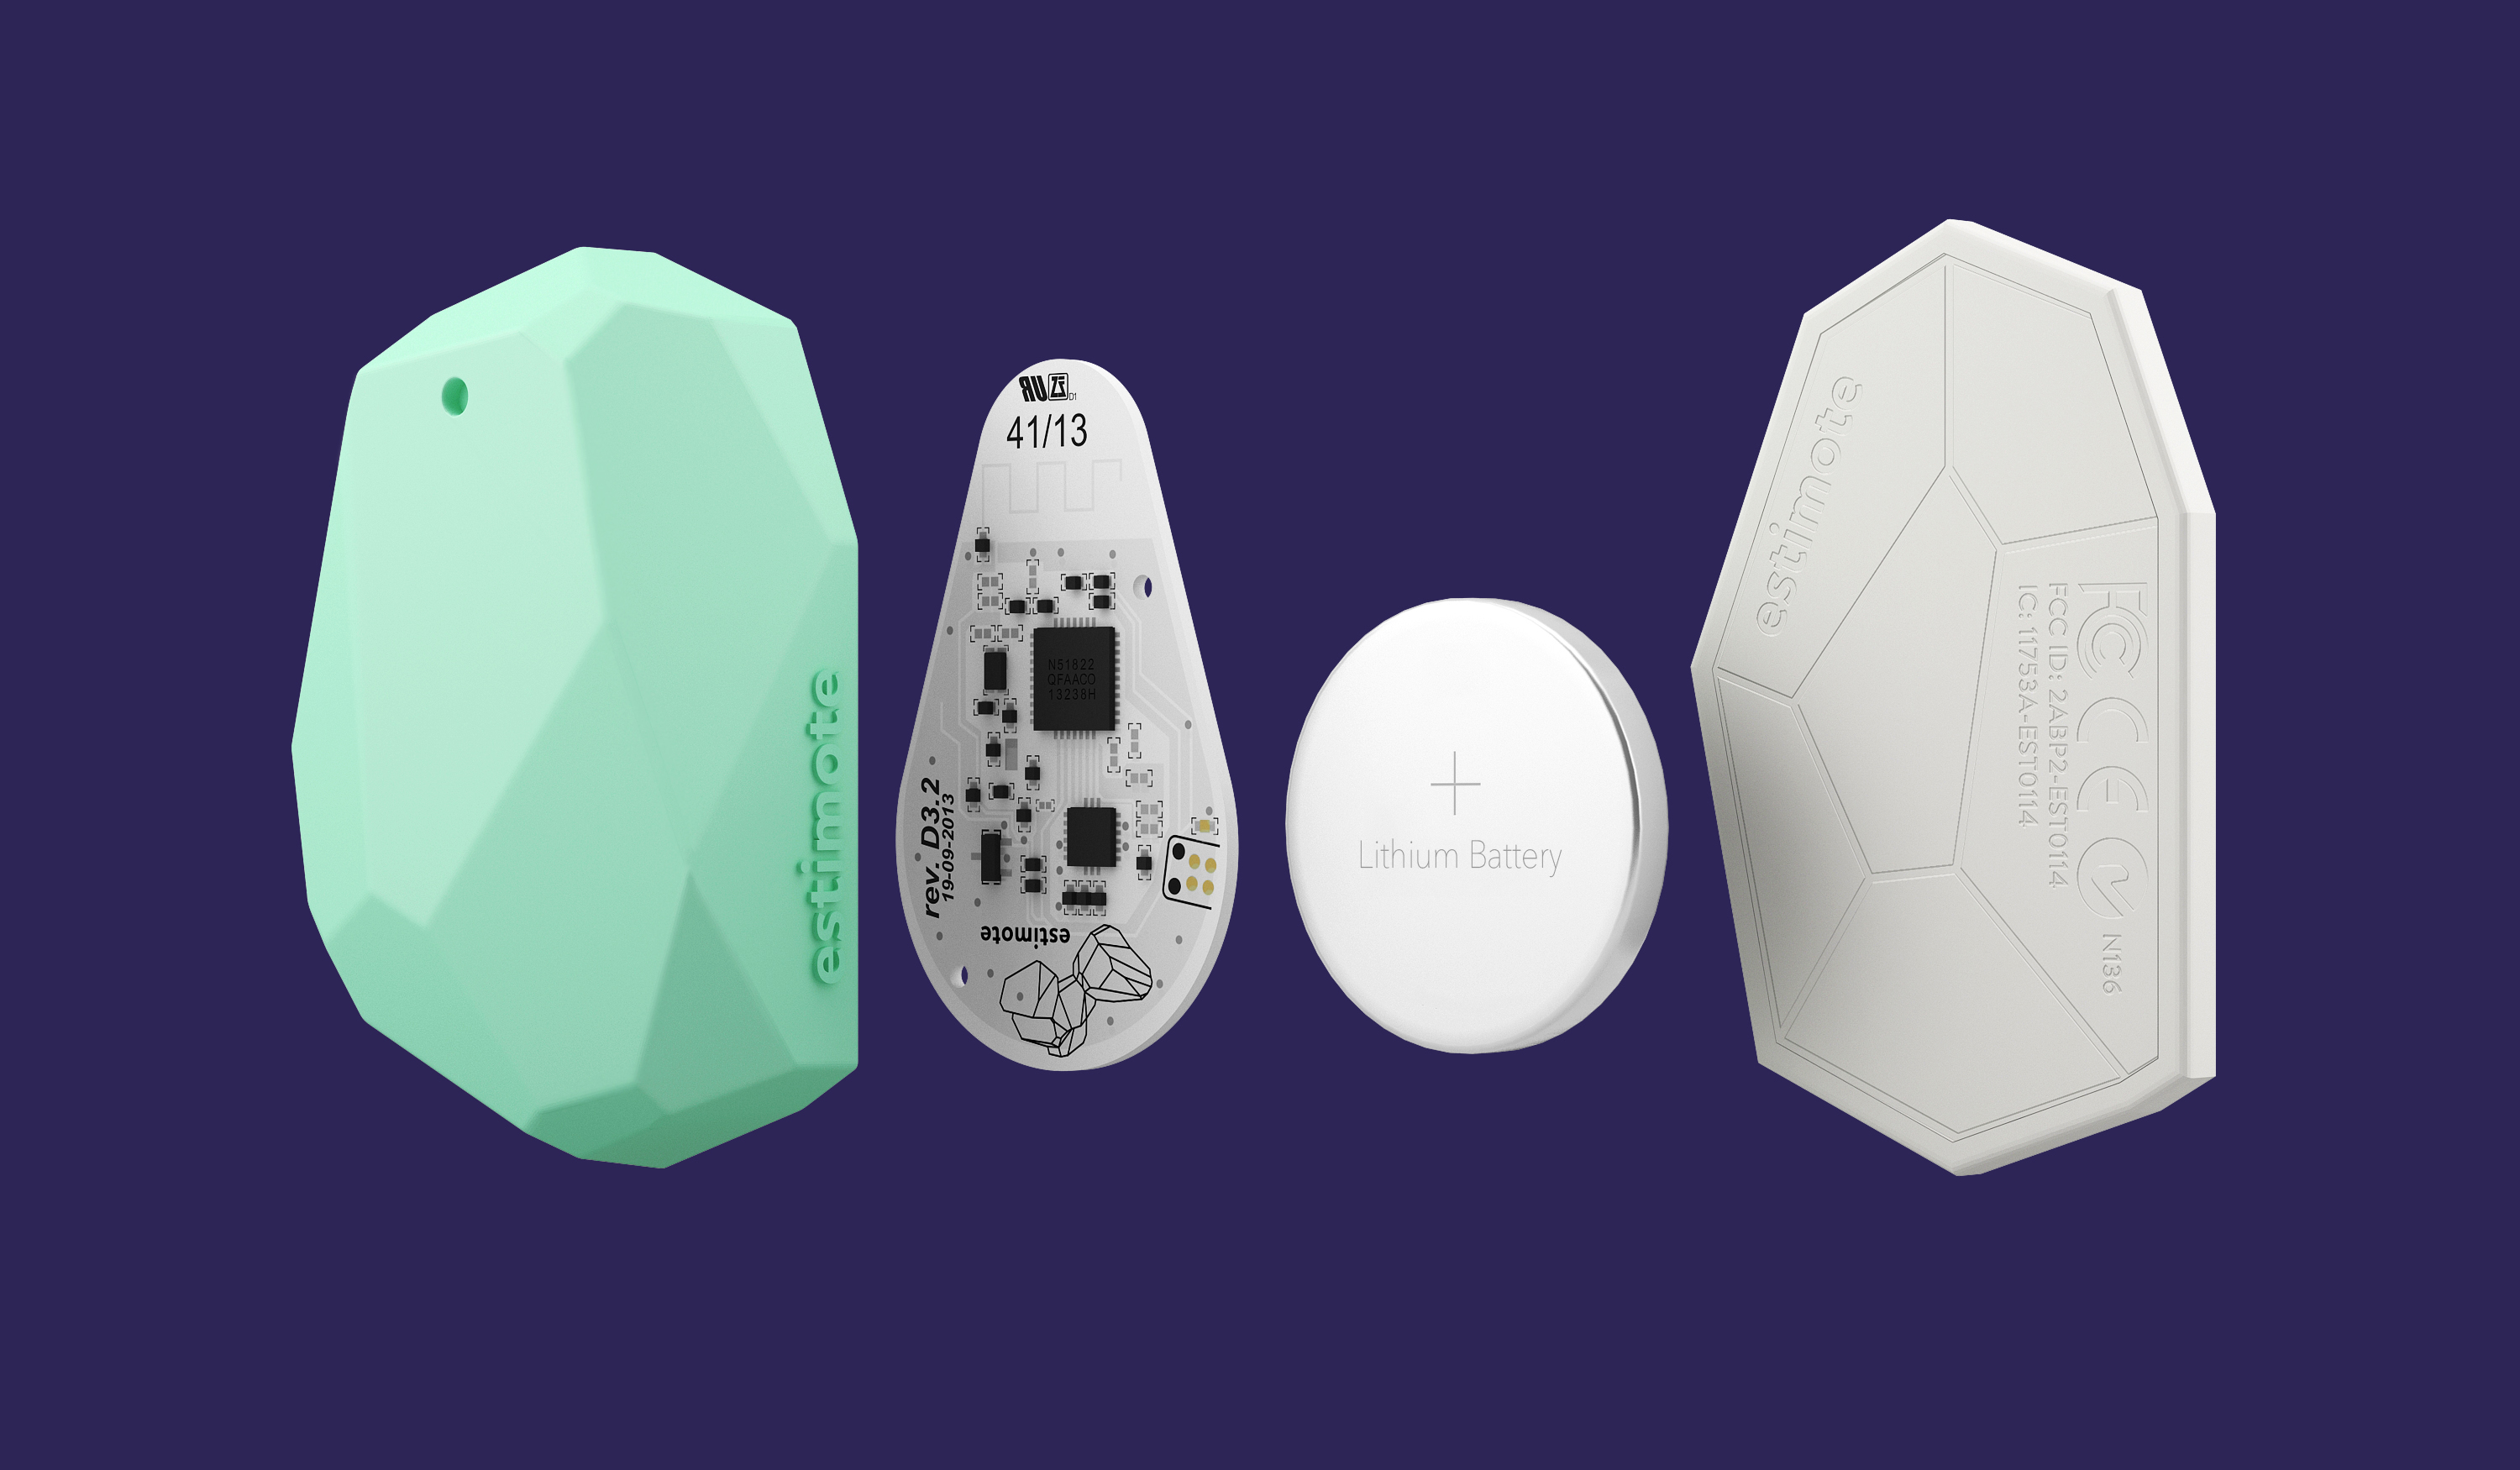
\includegraphics[width=1\textwidth]{estimote_beacons.jpg}
		\caption{The insides of an Estimote Bluetooth beacon. © by Estimote, Inc.}
	\end{center}
\end{figure}

\citep{bluetoothOverview} show that there are two roles for BLE devices, advertisers and scanners. Advertisers are devices that only transmit advertising packets through the advertisement channel in intervals of time. These intervals are called advertising events. Scanners on the other hand only receive packets from the advertisement channel. In the prototype application created for this thesis, the Bluetooth beacons are advertisers and the mobile phones are scanners. Some of the latest phones in the market are now also able to act as both the scanner and the advertiser. Therefore, this application could already be done without the need of separate Bluetooth beacons. However, there are only a handful of devices that are capable both roles, which results in the fact that this prototype application would be harder to test with a big group because the phones capable of it are still rare.

\citep{bluetoothOverview} also present findings that Bluetooth low energy consumes a lot of battery power which can be reduced by requesting data less frequently from the BLE device. This needs to be taken into account while using and developing the prototype application in order to make it as efficient as possible.

\section{Interviews}

This section describes the methods used for the interviews and the results gained from them. All interviews are anonymous and only basic demographic information about age and sex was gathered from the participants.

\subsection{Method for the interviews}

The interviews consist multiple open-ended questions. The goal is to find out information about how people behave while doing sports and what are their thoughts about the prototype application. The main questions for the interview are are located in appendix \ref{sec:app1_1}.

The questions aren't meant to be strict but just as a guideline for the discussion. If new interesting discussions emerge while interviewing, the idea is to go forward with them without thinking too much about the guideline.

The goal of the interviews was to do explorative research about possible directions for the design of the prototype application.

\subsection{Results}

In total, three people were interviewed for this thesis. A few demographic questions were included in the interviews. Two of the participants were female and one was  a male. One of the participants did sports four to five times a week, one two to three times a week and one did sports rarely (less than weekly). Their sports activities were gym, various group exercises (e.g. spinning), martial arts and jogging.

One of the participants was very goal oriented in their sports activities, others were doing spots just for getting a good feeling out of it. All of them carried devices for music during sports. Therefore, using the kind of a prototype application done for this thesis wouldn't require a change in their current behavior. Most of them did sports alone, sometimes together with friends. Friends that they did sports with, were mostly old friends from school. One of them got to know strangers that they frequently met at the gym and later started working out together.

Doing sports together with other people and alone had different effects to their motivation. One of the participants said that they didn't feel any difference in motivation when doing sports with or without friends. Others felt some differences.

\begin{quotation}
\it I might have a good motivation with or without friends. In a group settings, others are supporting me, which might make me achieve higher goals than I thought was possible. However, it might also end up so that we are just chatting without actually getting anything done. If I am working by myself, I try to gain motivation with some external factors (e.g. music or watching inspiring videos).
\end{quotation}

Privacy was a concern among the participants related to this prototype application. The initial thought for one of them was that strangers would start to stalk them using this kind of an application. One other participant quickly dismissed the idea by saying that of course showing any personal information should be voluntary. Some concerns were also brought up about criminals, such as pedofiles using this application for criminal activities. The same participant dismissed this idea also by saying that the application has no role in that situation if the people are actually meeting each other in real life all the time. However, initial reactions about privacy are important when designing an application that feels safe to use.

When asked about what they would be willing to share to strangers, the answers differed. One of them felt quite easy about sharing plenty of information.

\begin{quotation}
\it I would maybe be willing to share some open text related to my interests, my profile picture, my sex, my first name and maybe my email address. If it were a dating service and I would be actively searching for a partner, I would be willing to share more information.
\end{quotation}

One of the participant felt anxious about sharing a profile picture. One felt that profile pictures weren't necessary if the search is for a person to do sports with. Overall, they felt that the most important aspect would be to share an open field where one could describe what they are interested in and perhaps write about the kinds of people they are looking to do sports with. In addition, they felt that being optionally able to select a sex for the familiar strangers would be a good thing. They felt that most people would probably want to select a gender for people to interact and to do sports with.

\begin{quotation}
\it If I am looking for someone to spot me at the gym, I don't want it to be someone who weights 20kg or if a woman is searching for a yoga partner, they might feel more comfortable if the partner is female as well.
\end{quotation}

When asked, if they were willing to use the application to meet strangers to do sports with, the participants were hesitant.

\begin{quotation}
\it Possibly yes, if it were possible to find good people to work out with.
\end{quotation}

One of the participants said that they would be willing to use it if they were single, not otherwise. One of them said that they wouldn't use the application themselves but understand if others would want to.

Interviews of three people aren't enough to draw exact conclusions about whether this kind of social interaction enhanced by an application is something people are looking for. However, this interview yield some good directions for the application on what makes people anxious and how far boundaries can be pushed while maintaining an overall safe feeling for the application.


\section{Design}

The prototype application's main goal is to allow people to connect with familiar strangers and to find like-minded people to do sports with. Of course the underlying concepts can be used for other purposes than just sports, but this prototype is designed for sports. Especially part related to social interaction could be imported into a dating application for example. However, this thesis doesn't cover any other use cases for this prototype application.

The designed process of meeting a familiar strangers and connecting with them can be divided into a few steps.

\begin{itemize}
	\item Pass by the person enough times
	\item View information about the person and their interests when the application suggests communication.
	\item Message the stranger and see if they share common goals.
	\item View their real-life information after both agree to do it and start doing sports with them.
\end{itemize}

This prototype application is a mix of remote and local social interaction among people assisted by technology. Users are able to chat with familiar strangers remotely but real life proximity is required to initialize these conversations. The aim is to push the boundaries of how social interaction is initialized among strangers. In this prototype application, shared common interests are the starters for social interaction among strangers. The process is designed to be as smooth as possible in order to find new people to do sports with.

\subsection{Onboarding}

\begin{figure}[htb]
	\begin{center}
		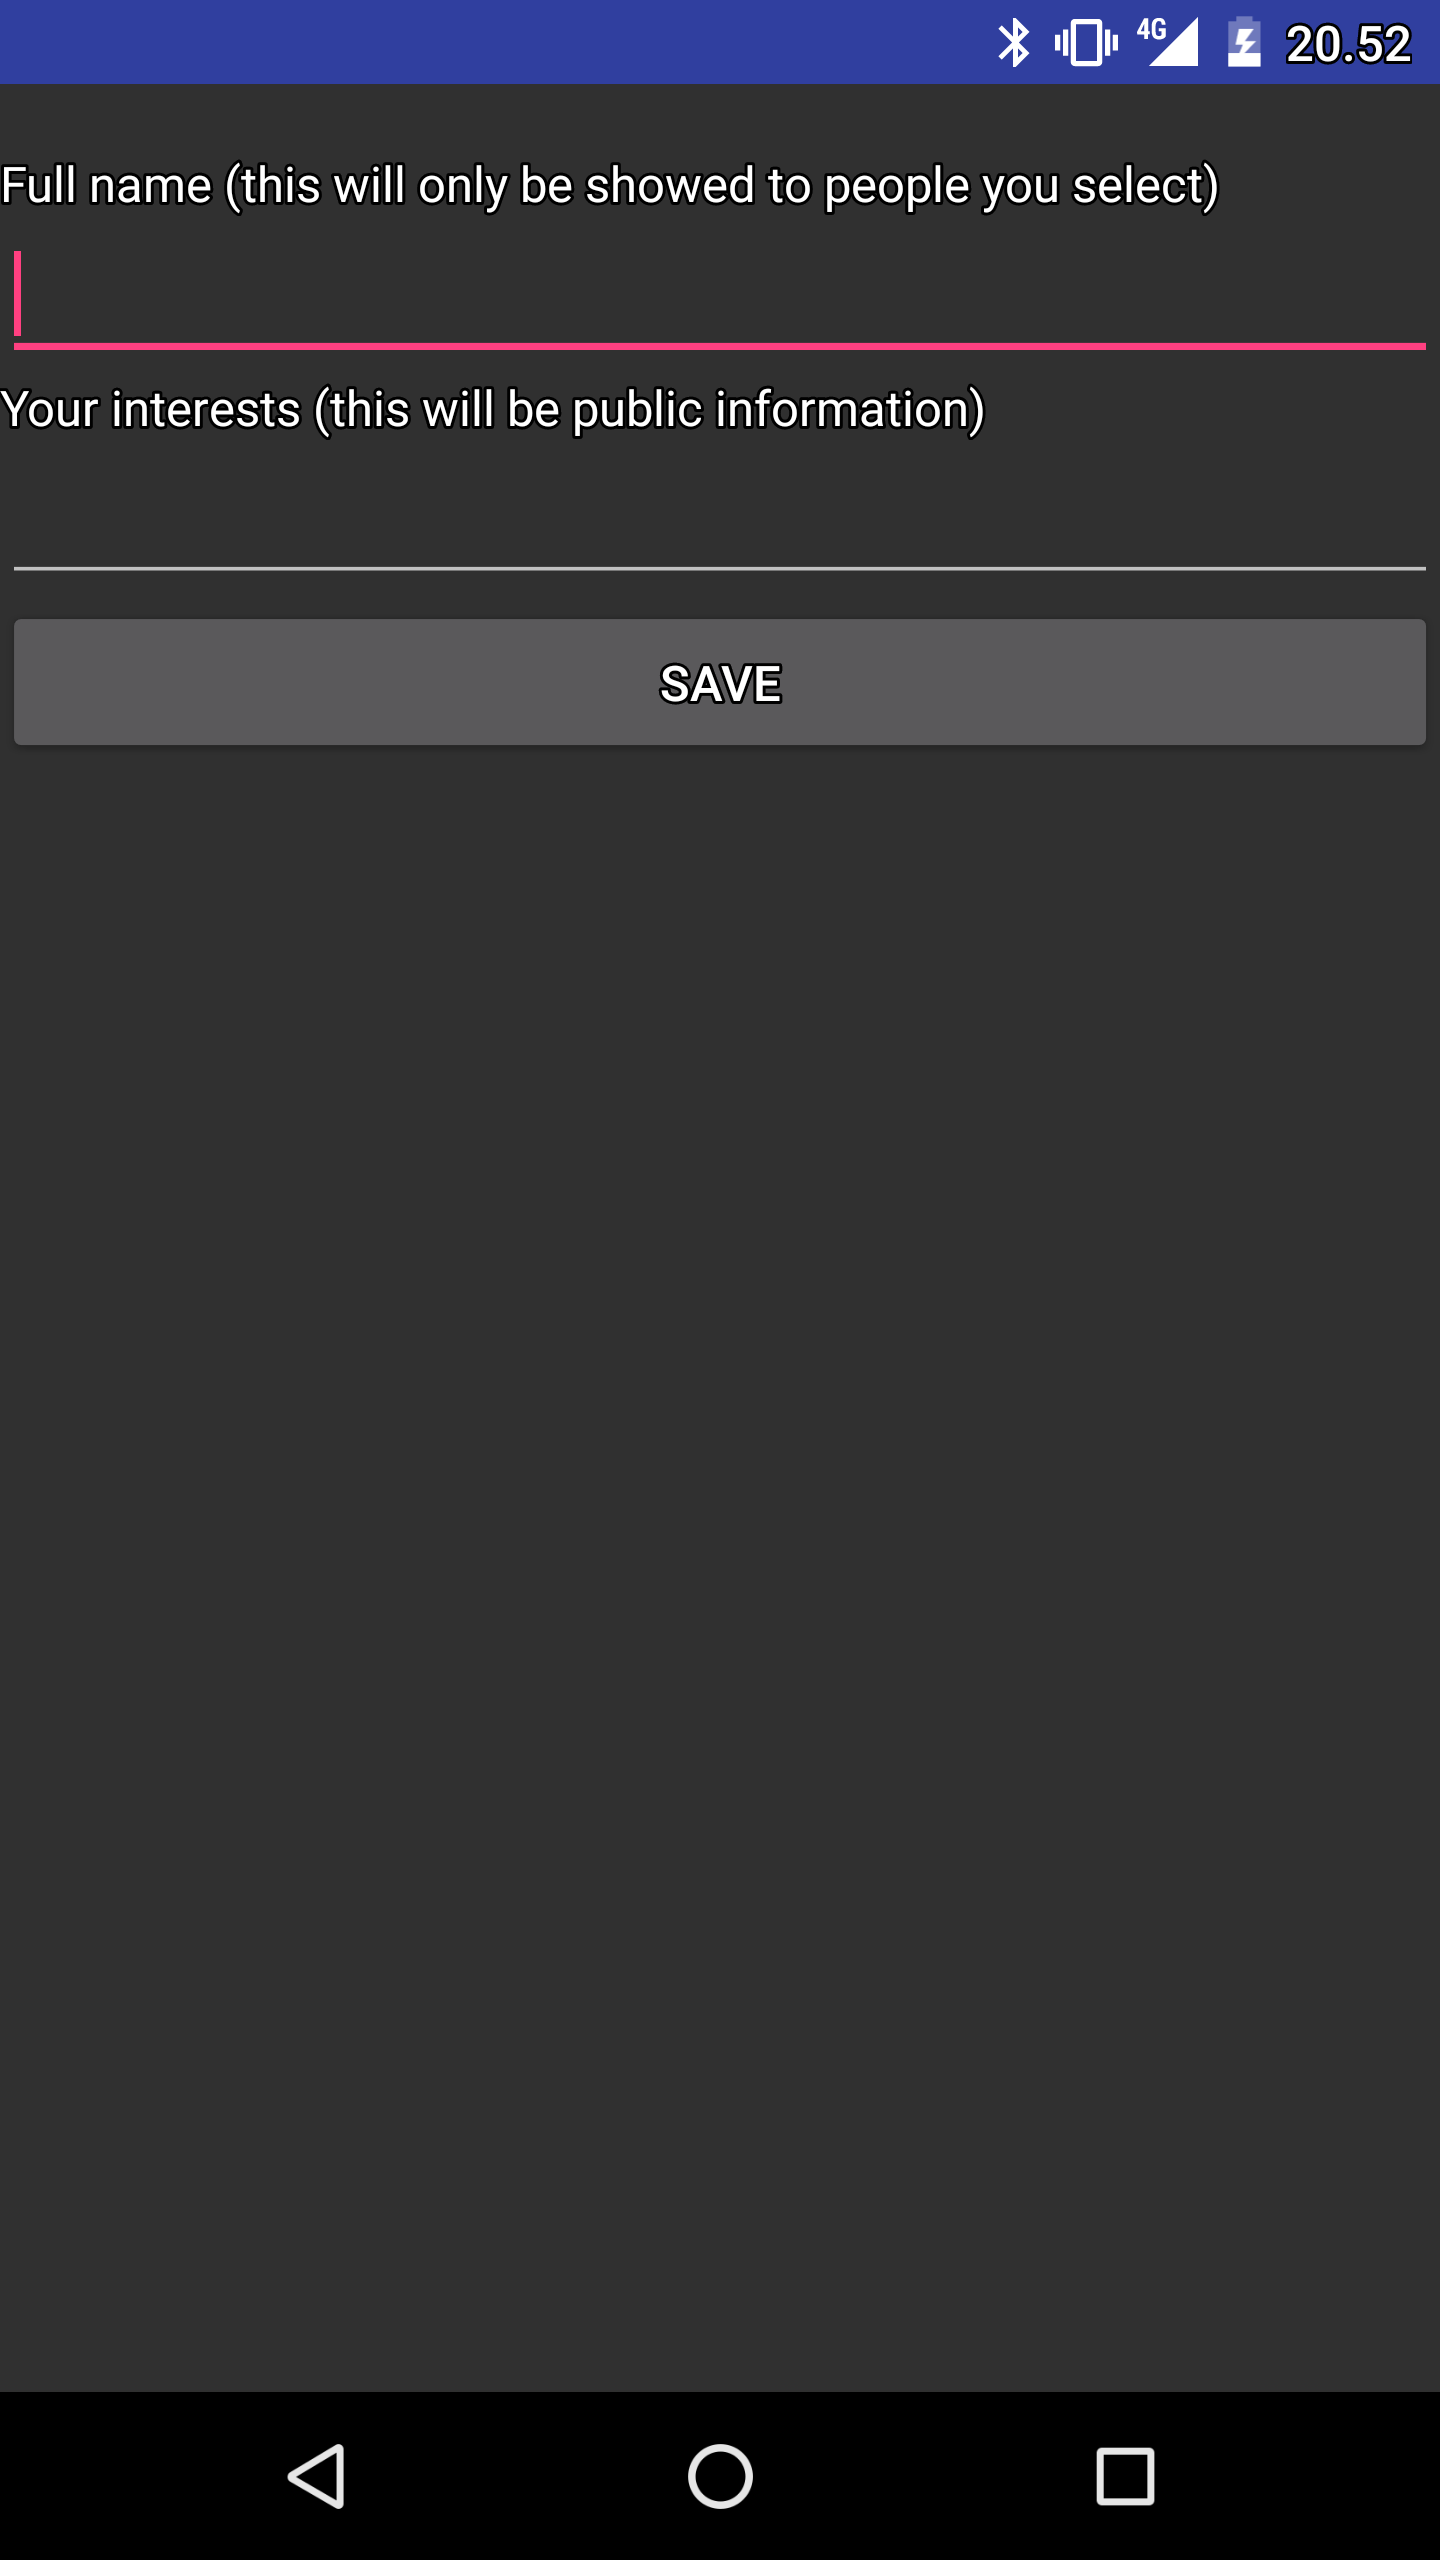
\includegraphics[width=0.4\textwidth]{fs_onboarding.png}
		\caption{Filling personal information.}
	\end{center}
\end{figure}

When starting the application for the first time an onboarding process will begin for the user. The user is required to register for the application. They can also just log in with an existing account so using the application isn't tied to a single device. After that the user is required to fill their profile information. The fields required for this are their name and public interests. After completing this stage of the onboarding the user is required to register a beacon for their use. At this point the application will detect every beacon nearby and show them in a list. Beacon's MAC address is used to identify unique beacons and it is stored to the server. Therefore, every beacon is tied to an identifiable user. This completes the onboarding process and the user is now free to use the application.

\subsection{Passing by}

Using Bluetooth beacons, the application will log every person that passes by. Only one of the users have to have their mobile phone with them, since all the encounters are stored in the server. Therefore, only carrying a Bluetooth beacon might end up resulting in encounters inside the application but it is not guaranteed. In the case where both users only have a beacon with them, no encounters will be stored. The amount of pass by's that initialize communication between the users is adjustable in the prototype for better examining of how much is required for social interaction later on. The initial default value is three times. This can easily be adjusted from the server later so no additional application releases need to be made. The amount could also in the future be adjusted based on how frequent the use of the application is in the area. With low use, it is harder to encounter anyone and likely will lead to not using the application as often. If a larger study is done later to validate the users behaviors, the amount should be increased to engage people more during the research process.

One option is also to modify the application so that the users are able to select the amount themselves before other users are able to approach them with messages. The option of filtering the strangers with some parameters, such as sex was brought up in the interviews. The conducted interview also suggested that users would be interested to see the public interests of strangers even with low encounters in order to find a like-minded stranger more easily.

\begin{figure}[htb]
	\begin{center}
		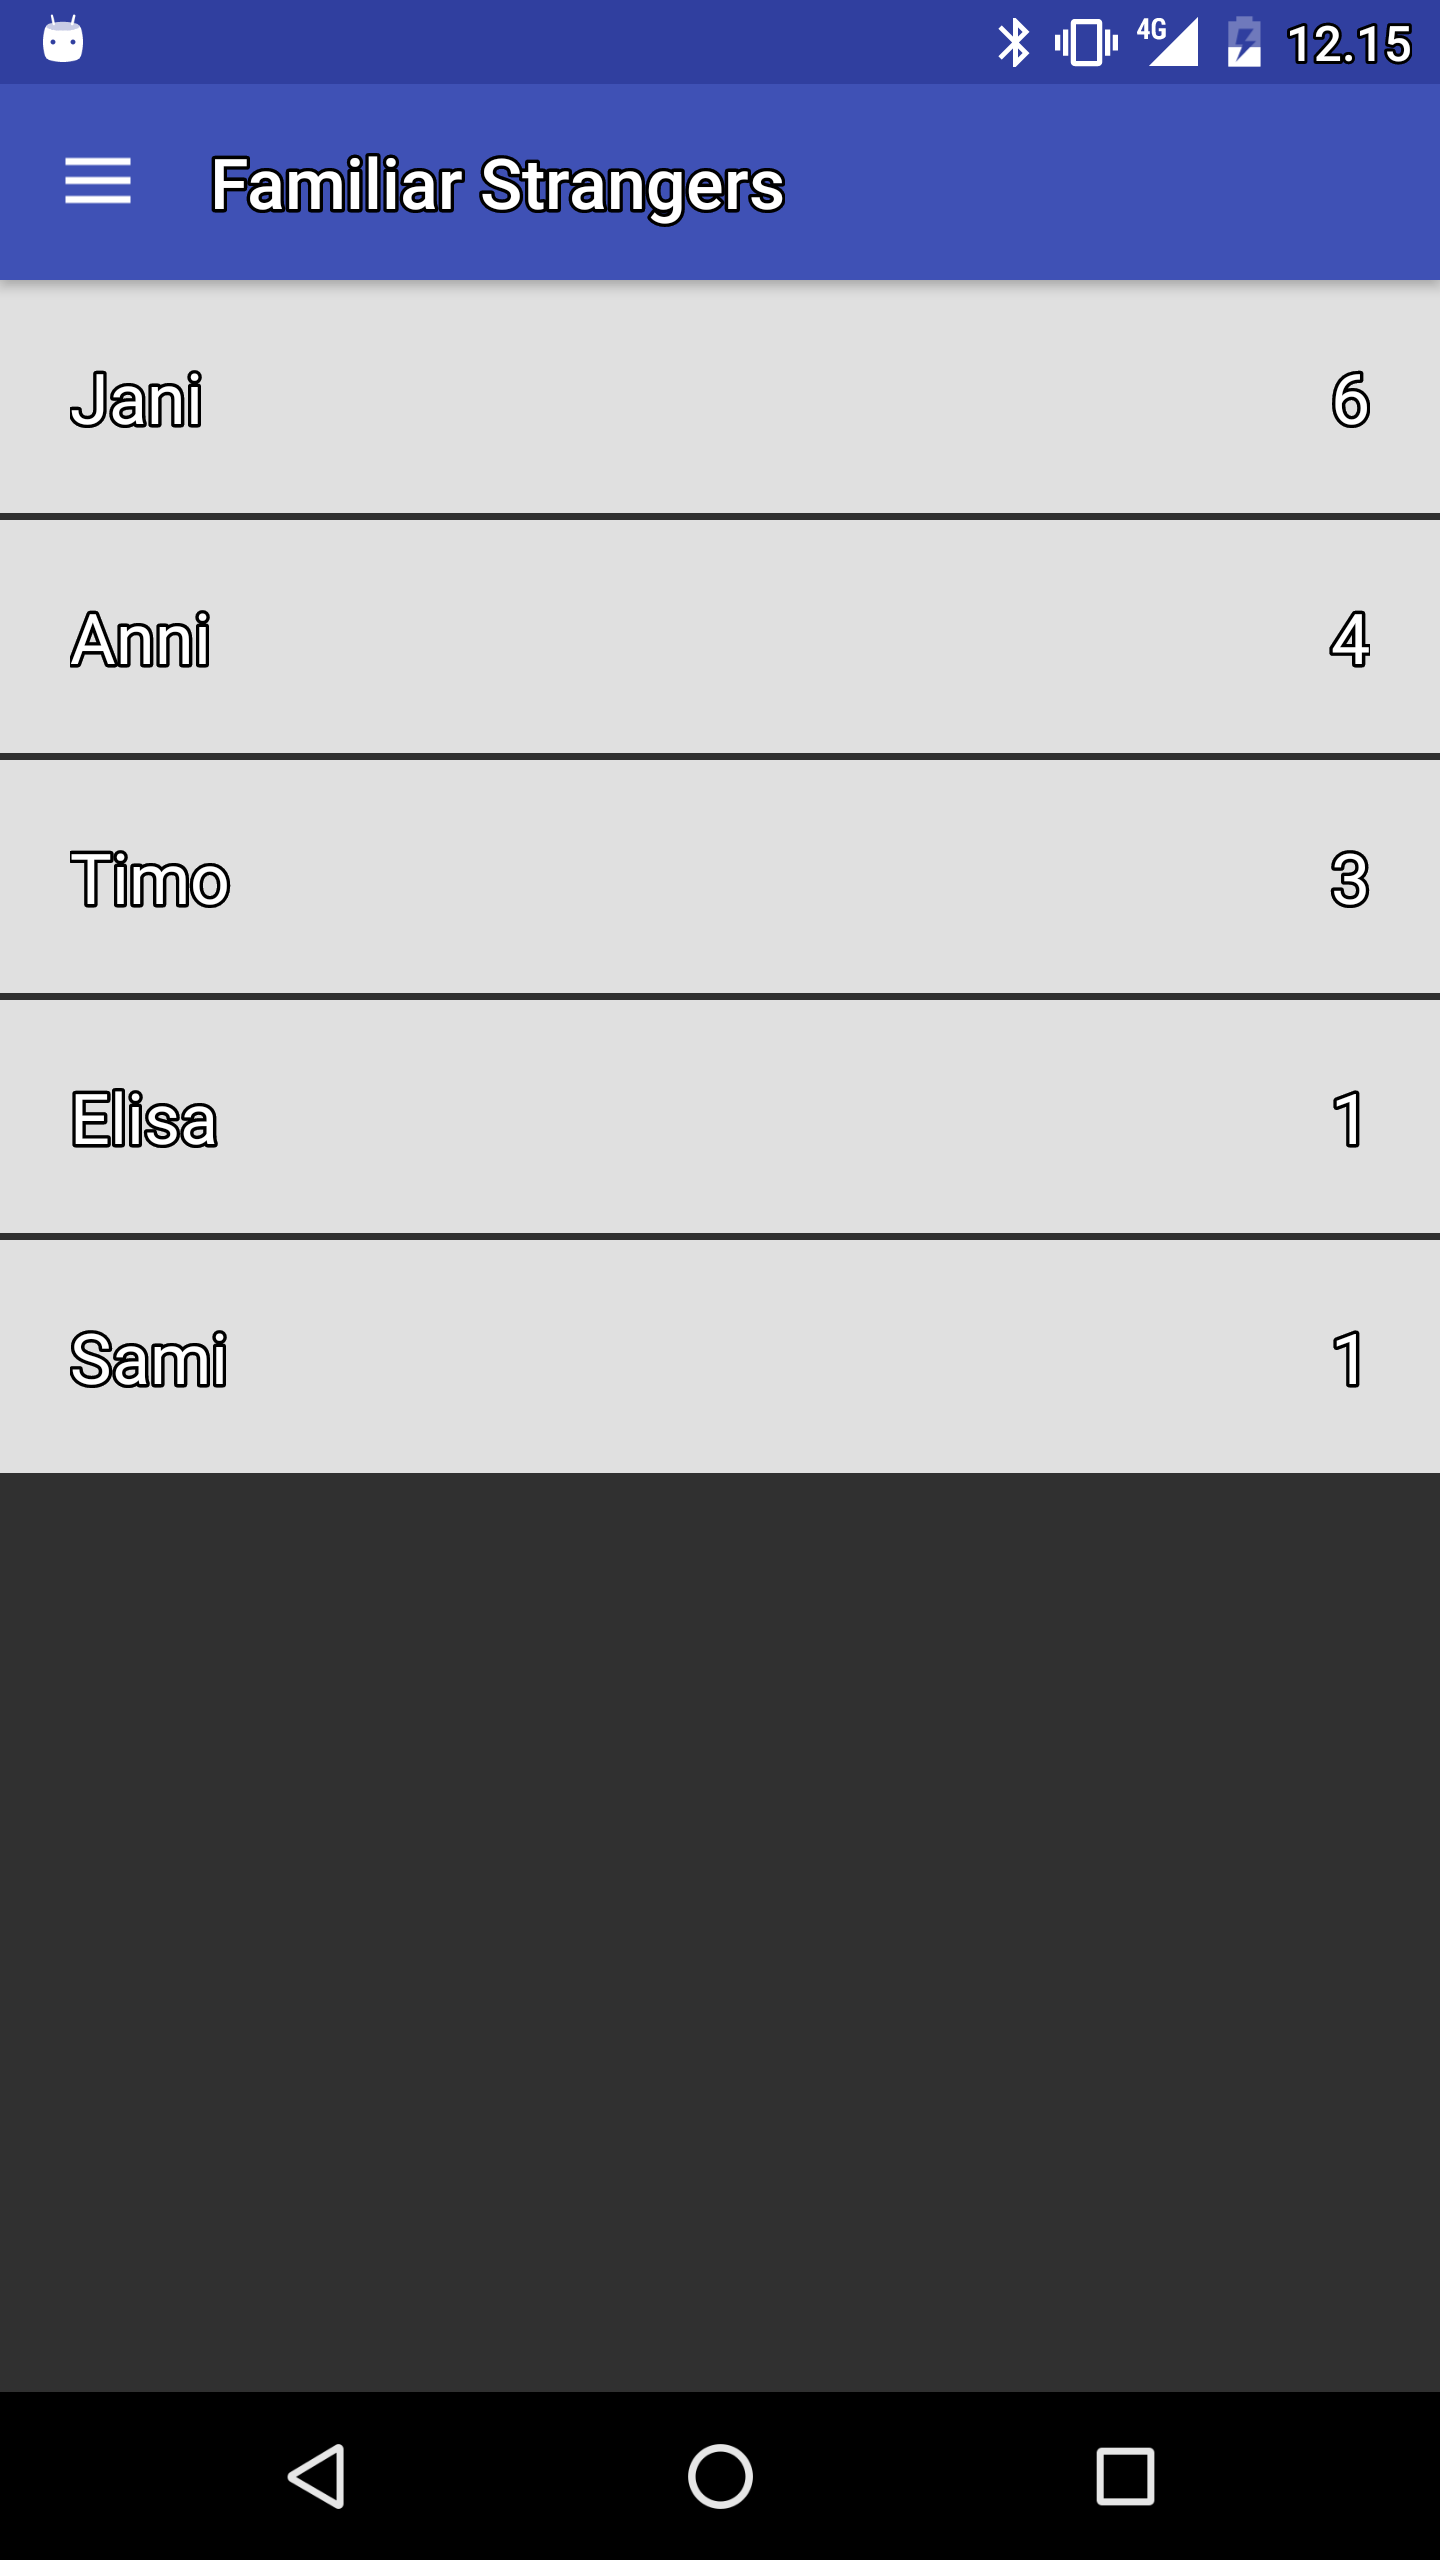
\includegraphics[width=0.4\textwidth]{encounters.png}
		\caption{A list of encounters (made up name and how many times)}	
	\end{center}
\end{figure}

%TODO make correct references to the figure.

In the application, users are able to view how many people they have come encountered from a list in the application as seen in Figure X. The list shows the user with an unique identification (not their real name) and also the times they have come across each other. These users have encountered the threshold of encounters. Strangers with less encounters than required will not be visible in any way to the user before reaching the target.

The logging can be turned on and off whenever the user feels like it. This is a requirement from the mobile application providers and also a feature requested in the conducted interviews. The reason could be that the user is in a place where they do not want to encounter anyone or have a record of the location stored in the application or if they want to save battery by closing every Bluetooth connection.

\subsection{Approaching the stranger}

After the user has encountered a familiar stranger enough times, the application will suggest communication between both parties. The user will be able to send messages and view their public interests that they have filled during the onboarding process. In addition to the filled information, the user is able to see the locations of encounters on a map, to make sense of where the other person is doing sports and what sports based on the users own behavior. 

%TODO Reference the correct paper.
Based on the literature review of this thesis and the interviews, displaying this kind of information publicly to the users shouldn't be a problem for the majority of users as users are open about reaching out to strangers.

The interaction can stay anonymous (with temporary names) as long as the users want to. The anonymity was selected based on the privacy concerns of the conducted interview. It's possible to send messages to each other just to ask what they are interested in and see if both of them would be interested in doing sports together. The chat is meant for users to verify similar interests and goals before getting to know each other better. If the interests and goals do not match, the user can ignore the other person and they will not be in any kind of interaction via the application ever again.

\subsection{Revealing identity}

At some point, the users must reveal some real life information in order to meet in person and to do sports with. This can be done only by messaging related information via the application. However, the application also introduces a feature, that the users can use to reveal real life information to one another. The real life information should be revealed only after both parties feel entirely comfortable with the idea. In the prototype, a mutual agreement of revealing real life information is required in order for it to happen. After revealing information, it is possible for both of them to start doing sports together or find other meaningful things to do in life. Their profiles in the application will now be visible with their real names. A record of their communication is left on the app, and it will not log any encounters from the other person anymore at this point. Until real life information is accepted, the application will still log encounters from the person and view them in the list of encounters unless the user chooses to remove them manually.

\section{Prototype implementation}

The created prototype is an Android\footnote{\url{https://www.android.com/}} application. The programming language selected for the application is Kotlin\footnote{\url{https://kotlinlang.org/}}. Kotlin helped to reduce the amount of bugs during the creation process and proved to be a very fast programming language for d	eveloping Android applications. Null safety by default, drastically less boilerplate code compared to a traditional Java application for Android and great development tools where the key elements for the success of using Kotlin. In addition to Kotlin, Anko\footnote{\url{https://github.com/Kotlin/anko}}; a view library created by JetBrains\footnote{\url{https://www.jetbrains.com/}}; was also used for the application. Using Anko reduced the amount of time going to creating basic views, e.g. for the login and registering views.

\subsection{Architecture}

\begin{figure}[htb]
	\begin{center}
		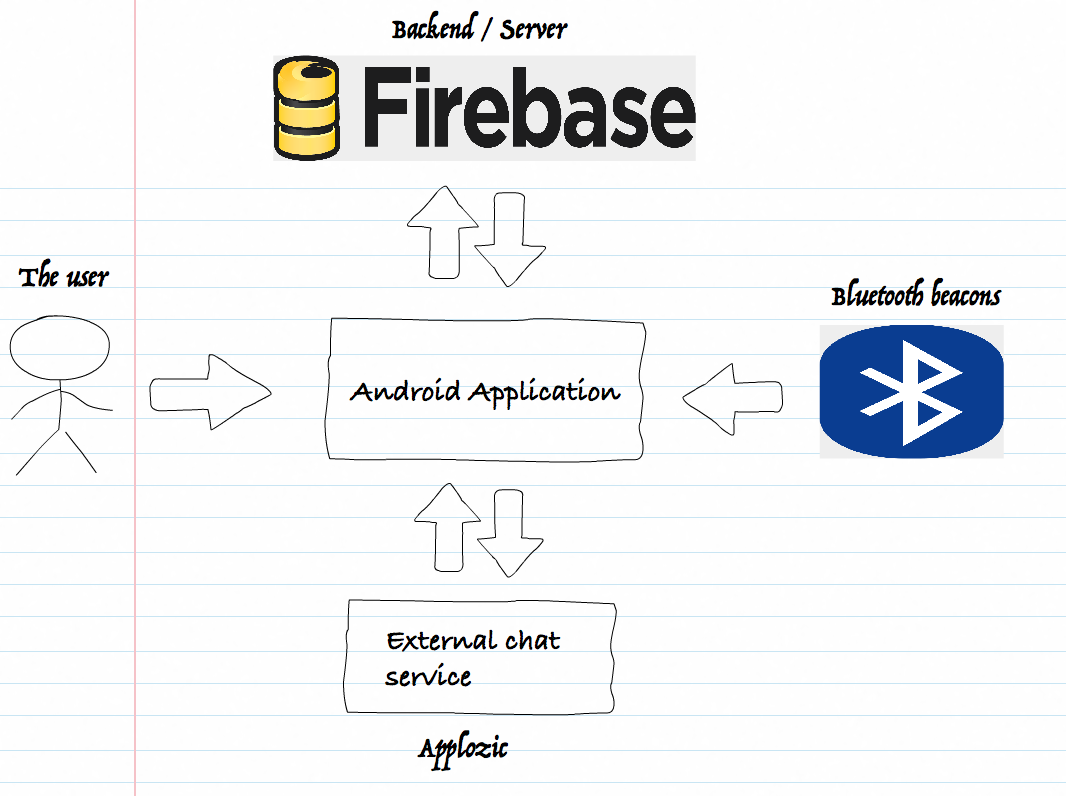
\includegraphics[width=1\textwidth]{fs_architecture.png}
		\caption{The application architecture.}	
	\end{center}
\end{figure}

%TODO reference the correct figure.
The main parts of the prototype application are the client (the Android application) and the backend (server) as demonstrated in figure X. The backend is built with Firebase\footnote{\url{https://www.firebase.com/}}, which is a tool for creating fast backends using nothing but JSON\footnote{Javascript Object Notation} objects. The user authenticates to the backend, so that we get unique users ID's that aren't locked into a single device in the application's lifetime. In addition to Firebase, the application uses an external chat service for the messaging feature.

The application uses Firebase's default authentication features for the authentication. A combination of email and password is currently used. However, it is easy to add third party login systems, such as Facebook\footnote{\url{https://www.facebook.com/}} and Google\footnote{\url{https://www.google.com}} for the authentication.

The application uses a background service to run the logging of encounters among the users in a separate thread. The background service detects the join and exit events of Bluetooth beacons and based on those events, sends the server information about the encounters. This background service will stay running even though the user is not currently actively using the application. Monitoring the events for Bluetooth beacons drains extra battery from the phones as described by \citep{bluetoothOverview}.

Push notifications are not at the moment handled by a real-time push notification server. The application polls the Firebase server periodically and sees if there are any changes available. This will hopefully be improved in the future. The external chat service has push notifications enabled, but this is a different system to the applications own backend. Therefore, push notifications work for the messaging feature but nothing else.

\subsection{Using the prototype}

The application is open sourced with the Apache 2.0 license\footnote{\url{http://www.apache.org/licenses/LICENSE-2.0}}. Therefore, anyone is free to take it into use, modify it or even make money out of it. A few steps are needed before the application can be taken into use by someone. First of all, the application uses Firebase as the backend service. Therefore, a Firebase account and an application created with it is required for using this application. The data structure for the JSON objects used in Firebase is described in the appliation's source code, so developing a custom backend for the application is entirely possible and quite fast to do.

\section{Discussion}

This section analyses the results that the study produced and what should be done in the future related to the created prototype application and about researching the social interactions of familiar strangers.

\subsection{Results of the study}

The literature review of the application showed that social sports applications have been studied to increase social interaction even in completely remote and virtual environments. In addition, to social sports it was shown that doing sports together with other people facilitates social interaction among the people. Therefore, the basis for the application's premises is well researched.

The conducted interviews presented multiple interesting points of views. However, as the amount of interviews is so low, it is not possible to draw general conclusions about the behavior models of users. The results served their purpose in giving general direction to the prototype application's design process and therefore resulted in very valuable information for this study.

The prototype application is functional and it its possible to use it for further research. The application is also open source with a permissive license so it's easy to take it into use in any research facility or even commercial use.

\subsection{Future work}

A larger study should be conducted to validate the behavior models and assumptions that were generated by the conducted interviews. In addition to researching the behavior models of doing social interaction among familiar strangers, the prototype application should be used for more and larger research. Elements of this prototype application could also be introduced outside the concept of sports in order to research whether there are any differences in the behavior of these groups.

It might be best to conduct research with this application in a certain geographical area such as an university campus or a regular neighborhood. Then it is more likely that encounters will happen as real life proximity is required for them.

Some additional functionality is planned for the application. The proposed features are listed in the GitHub page of the application. At this point it is unclear whether those features will be implemented, but they are there for anyone to take. Modifications to the code and complete new features are by all means welcome and will be merged to the prototype application.

No user testing has been done for this prototype application. However, as the application is licensed with an open source license, hopefully a study will see the light of day sometime in the near future.

% --------------------------------------------------------------------
